\documentclass[tikz,border=0pt]{standalone}
\usepackage{xcolor}
\usetikzlibrary{calc}
% Palette: Sam_Comm_final.png by eye (vagrancy repository).
\definecolor{ink}{HTML}{3B2340}
\definecolor{dark}{HTML}{4A3357}
\definecolor{darkhi}{HTML}{5E4A6E}
\definecolor{sky}{HTML}{EFC46A}
\definecolor{skyhi}{HTML}{F5DA92}
\definecolor{skylow}{HTML}{E9B060}
\definecolor{cloud}{HTML}{F2D58A}
\definecolor{wallA}{HTML}{E88A73}
\definecolor{wallB}{HTML}{EE9F7E}
\definecolor{wallC}{HTML}{E47A7E}
\definecolor{wallD}{HTML}{F0B07E}
\definecolor{wallE}{HTML}{D9765F}
\definecolor{wallF}{HTML}{E99A8A}
\definecolor{greenA}{HTML}{8DBB7E}
\definecolor{greenB}{HTML}{6FA77A}
\definecolor{greenC}{HTML}{A9C97F}
\definecolor{greenD}{HTML}{5E9C6A}
\definecolor{window}{HTML}{F6E7A0}
\definecolor{windark}{HTML}{8C5A64}
\definecolor{plum}{HTML}{8A5A9E}
\definecolor{plumhi}{HTML}{A77BB8}
\definecolor{lilac}{HTML}{D9C3E0}
\definecolor{coral}{HTML}{E47A7E}
\definecolor{coraldk}{HTML}{C85F65}
\definecolor{orange}{HTML}{F26B38}
\definecolor{salmon}{HTML}{F4BE9C}
\definecolor{gold}{HTML}{F2B53A}
\definecolor{golddk}{HTML}{D9962A}
\definecolor{butter}{HTML}{F5DA92}
\definecolor{cream}{HTML}{FFF4E0}
\definecolor{paper}{HTML}{F6E7C4}
\definecolor{sage}{HTML}{8DBB7E}
\definecolor{sagedk}{HTML}{6FA77A}
\definecolor{forest}{HTML}{5E9C6A}
\definecolor{mint}{HTML}{C5E0B4}
\definecolor{teal}{HTML}{5FA8A0}
\definecolor{glass}{HTML}{A9D3C9}
\definecolor{glassdk}{HTML}{7FB7B0}
\definecolor{pink}{HTML}{F2A7B5}
\definecolor{rosewall}{HTML}{F3B7A8}
\definecolor{steel}{HTML}{C8C2B4}
\definecolor{steeldk}{HTML}{8D9A93}
\definecolor{metal}{HTML}{8D9A93}
\definecolor{wood}{HTML}{B9835A}
\definecolor{wooddk}{HTML}{8E5E3C}
\definecolor{tan}{HTML}{E2BD8C}
\definecolor{paving}{HTML}{E2BD8C}
\definecolor{ground}{HTML}{D3A77D}
% One ink for every outline.
\newcommand{\Ink}{1.3pt}
\tikzset{inked/.style={draw=ink, line width=\Ink, line join=round, line cap=round}}
% Picture units: 0.4 mm, y counted downward (hence the negative y unit).
\tikzset{x=0.4mm, y=-0.4mm}
\begin{document}
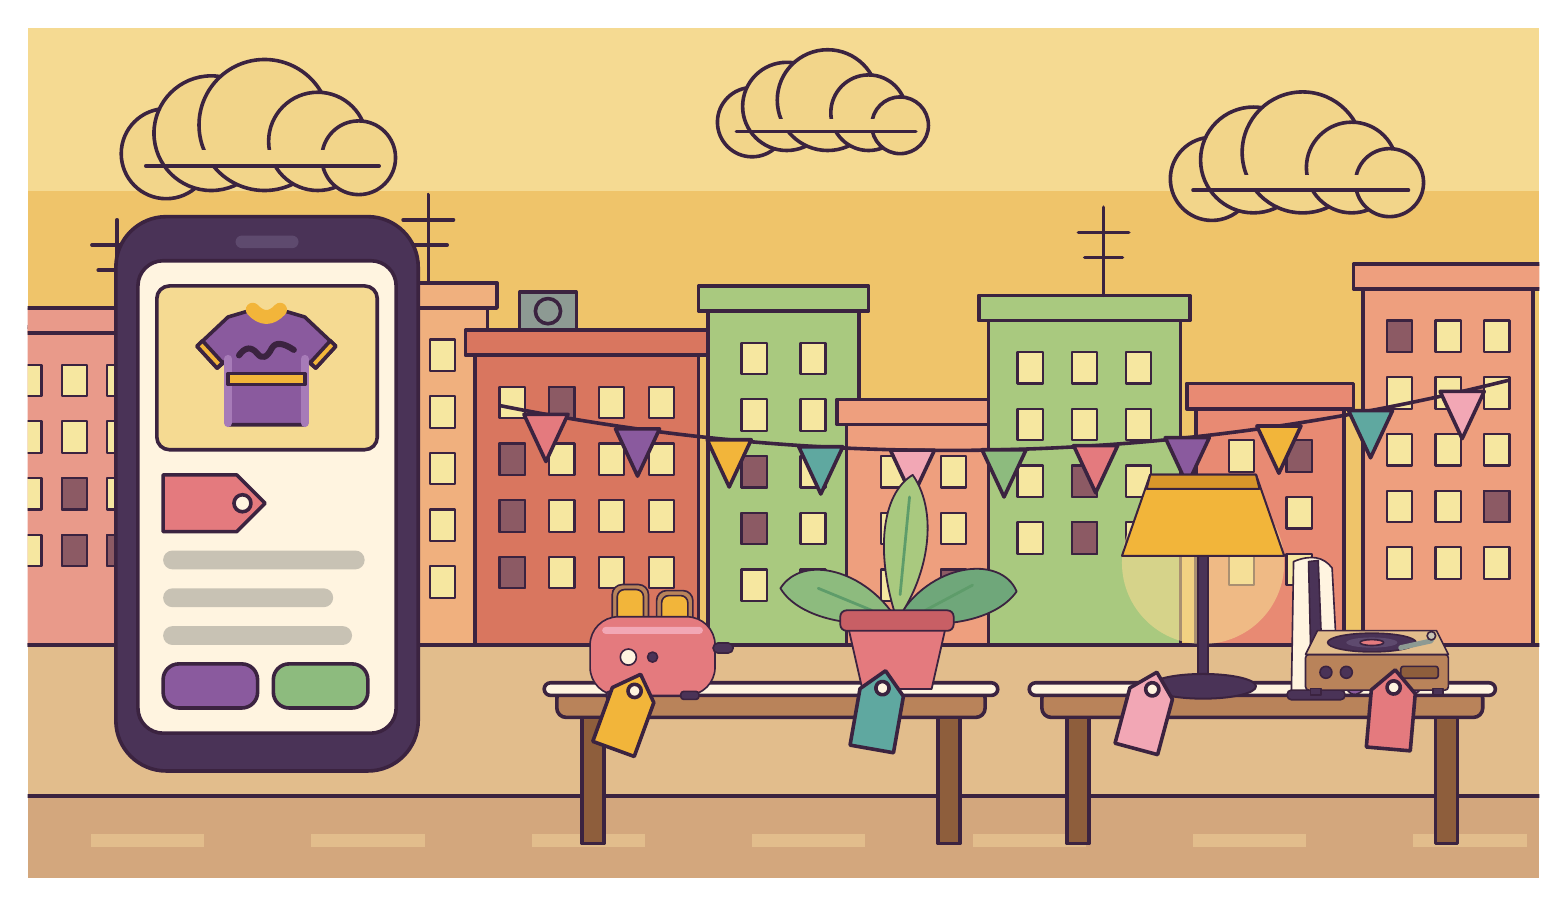
\begin{tikzpicture}
\clip (0,0) rectangle (480,270);
% sky and clouds
\fill[sky] (0,0) rectangle (480,270);
\fill[skyhi] (0,0) rectangle (480,52);
\filldraw[inked,fill=cloud] (44,40) circle [radius=14.3];
\filldraw[inked,fill=cloud] (58.3,33.5) circle [radius=18.2];
\filldraw[inked,fill=cloud] (75.2,30.9) circle [radius=20.8];
\filldraw[inked,fill=cloud] (92.1,36.1) circle [radius=15.6];
\filldraw[inked,fill=cloud] (105.1,41.3) circle [radius=11.7];
\fill[cloud] (44,38.7) rectangle (105.1,43.9);
\draw[ink, line width=1.3pt, line cap=round, line join=round] (37.5,43.9) -- (111.6,43.9);
\filldraw[inked,fill=cloud] (230,30) circle [radius=11];
\filldraw[inked,fill=cloud] (241,25) circle [radius=14];
\filldraw[inked,fill=cloud] (254,23) circle [radius=16];
\filldraw[inked,fill=cloud] (267,27) circle [radius=12];
\filldraw[inked,fill=cloud] (277,31) circle [radius=9];
\fill[cloud] (230,29) rectangle (277,33);
\draw[ink, line width=1.3pt, line cap=round, line join=round] (225,33) -- (282,33);
\filldraw[inked,fill=cloud] (376,48) circle [radius=13.2];
\filldraw[inked,fill=cloud] (389.2,42) circle [radius=16.8];
\filldraw[inked,fill=cloud] (404.8,39.6) circle [radius=19.2];
\filldraw[inked,fill=cloud] (420.4,44.4) circle [radius=14.4];
\filldraw[inked,fill=cloud] (432.4,49.2) circle [radius=10.8];
\fill[cloud] (376,46.8) rectangle (432.4,51.6);
\draw[ink, line width=1.3pt, line cap=round, line join=round] (370,51.6) -- (438.4,51.6);
% buildings
\filldraw[inked,fill=wallF] (-10,95) rectangle (54,196);
\filldraw[inked,fill=wallF] (-13,89) rectangle (57,97);
\foreach \i in {0,...,3} \foreach \j in {0,...,3} \filldraw[inked, line width=0.8pt, fill=window] (-3.6+\i*14.4,107+\j*18) rectangle ++(8,10);
\filldraw[inked, line width=0.8pt, fill=windark] (39.6,143) rectangle ++(8,10);
\filldraw[inked, line width=0.8pt, fill=windark] (10.8,161) rectangle ++(8,10);
\filldraw[inked, line width=0.8pt, fill=windark] (10.8,143) rectangle ++(8,10);
\filldraw[inked, line width=0.8pt, fill=windark] (25.2,161) rectangle ++(8,10);
\draw[ink, line width=1.3pt, line cap=round, line join=round] (28.4,89) -- (28.4,61) (20.4,69) -- (36.4,69) (22.4,77) -- (34.4,77);
\filldraw[inked,fill=wallF] (52,111) rectangle (96,196);
\filldraw[inked,fill=wallF] (49,105) rectangle (99,113);
\foreach \i in {0,...,1} \foreach \j in {0,...,2} \filldraw[inked, line width=0.8pt, fill=window] (61.33+\i*17.33,123+\j*18) rectangle ++(8,10);
\filldraw[inked, line width=0.8pt, fill=windark] (78.67,123) rectangle ++(8,10);
\filldraw[inked,fill=wallD] (99,87) rectangle (146,196);
\filldraw[inked,fill=wallD] (96,81) rectangle (149,89);
\foreach \i in {0,...,1} \foreach \j in {0,...,4} \filldraw[inked, line width=0.8pt, fill=window] (109.33+\i*18.33,99+\j*18) rectangle ++(8,10);
\filldraw[inked, line width=0.8pt, fill=windark] (109.33,135) rectangle ++(8,10);
\filldraw[inked, line width=0.8pt, fill=windark] (109.33,135) rectangle ++(8,10);
\draw[ink, line width=1.3pt, line cap=round, line join=round] (127.2,81) -- (127.2,53) (119.2,61) -- (135.2,61) (121.2,69) -- (133.2,69);
\filldraw[inked,fill=wallE] (142,102) rectangle (213,196);
\filldraw[inked,fill=wallE] (139,96) rectangle (216,104);
\foreach \i in {0,...,3} \foreach \j in {0,...,3} \filldraw[inked, line width=0.8pt, fill=window] (149.8+\i*15.8,114+\j*18) rectangle ++(8,10);
\filldraw[inked, line width=0.8pt, fill=windark] (149.8,132) rectangle ++(8,10);
\filldraw[inked, line width=0.8pt, fill=windark] (165.6,114) rectangle ++(8,10);
\filldraw[inked, line width=0.8pt, fill=windark] (149.8,150) rectangle ++(8,10);
\filldraw[inked, line width=0.8pt, fill=windark] (149.8,168) rectangle ++(8,10);
\filldraw[inked,fill=metal] (156.2,84) rectangle (174.2,96);
\filldraw[inked,fill=steeldk] (165.2,90) circle [radius=4];
\filldraw[inked,fill=greenC] (216,88) rectangle (264,196);
\filldraw[inked,fill=greenC] (213,82) rectangle (267,90);
\foreach \i in {0,...,1} \foreach \j in {0,...,4} \filldraw[inked, line width=0.8pt, fill=window] (226.67+\i*18.67,100+\j*18) rectangle ++(8,10);
\filldraw[inked, line width=0.8pt, fill=windark] (226.67,154) rectangle ++(8,10);
\filldraw[inked, line width=0.8pt, fill=windark] (226.67,136) rectangle ++(8,10);
\filldraw[inked,fill=wallB] (260,124) rectangle (309,196);
\filldraw[inked,fill=wallB] (257,118) rectangle (312,126);
\foreach \i in {0,...,1} \foreach \j in {0,...,2} \filldraw[inked, line width=0.8pt, fill=window] (271+\i*19,136+\j*18) rectangle ++(8,10);
\filldraw[inked, line width=0.8pt, fill=windark] (290,172) rectangle ++(8,10);
\filldraw[inked,fill=greenC] (305,91) rectangle (366,196);
\filldraw[inked,fill=greenC] (302,85) rectangle (369,93);
\foreach \i in {0,...,2} \foreach \j in {0,...,3} \filldraw[inked, line width=0.8pt, fill=window] (314.25+\i*17.25,103+\j*18) rectangle ++(8,10);
\filldraw[inked, line width=0.8pt, fill=windark] (331.5,157) rectangle ++(8,10);
\filldraw[inked, line width=0.8pt, fill=windark] (331.5,157) rectangle ++(8,10);
\filldraw[inked, line width=0.8pt, fill=windark] (331.5,139) rectangle ++(8,10);
\draw[ink, line width=1.3pt, line cap=round, line join=round] (341.6,85) -- (341.6,57) (333.6,65) -- (349.6,65) (335.6,73) -- (347.6,73);
\filldraw[inked,fill=wallA] (371,119) rectangle (418,196);
\filldraw[inked,fill=wallA] (368,113) rectangle (421,121);
\foreach \i in {0,...,1} \foreach \j in {0,...,2} \filldraw[inked, line width=0.8pt, fill=window] (381.33+\i*18.33,131+\j*18) rectangle ++(8,10);
\filldraw[inked, line width=0.8pt, fill=windark] (399.67,131) rectangle ++(8,10);
\filldraw[inked,fill=wallB] (424,81) rectangle (478,196);
\filldraw[inked,fill=wallB] (421,75) rectangle (481,83);
\foreach \i in {0,...,2} \foreach \j in {0,...,4} \filldraw[inked, line width=0.8pt, fill=window] (431.5+\i*15.5,93+\j*18) rectangle ++(8,10);
\filldraw[inked, line width=0.8pt, fill=windark] (431.5,93) rectangle ++(8,10);
\filldraw[inked, line width=0.8pt, fill=windark] (462.5,147) rectangle ++(8,10);
\filldraw[inked, line width=0.8pt, fill=windark] (462.5,147) rectangle ++(8,10);
% pavement
\fill[paving] (0,196) rectangle (480,270);
\draw[ink, line width=1.3pt, line cap=round, line join=round] (0,196) -- (480,196);
\fill[ground] (0,244) rectangle (480,270);
\draw[ink, line width=1.3pt, line cap=round, line join=round] (0,244) -- (480,244);
\foreach \dx in {20,90,...,480} \fill[tan] (\dx,256) rectangle ++(36,4);
% bunting over the yard sale
\draw[ink, line width=1.3pt, line cap=round, line join=round] (150,120) .. controls (256.67,141.33) and (363.33,138.67) .. (470,112);
\filldraw[inked,fill=coral] (157.55,122.76) -- (171.55,122.76) -- (164.55,137.76) -- cycle;
\filldraw[inked,fill=plum] (186.64,127.39) -- (200.64,127.39) -- (193.64,142.39) -- cycle;
\filldraw[inked,fill=gold] (215.73,130.83) -- (229.73,130.83) -- (222.73,145.83) -- cycle;
\filldraw[inked,fill=teal] (244.82,133.07) -- (258.82,133.07) -- (251.82,148.07) -- cycle;
\filldraw[inked,fill=pink] (273.91,134.13) -- (287.91,134.13) -- (280.91,149.13) -- cycle;
\filldraw[inked,fill=sage] (303,134) -- (317,134) -- (310,149) -- cycle;
\filldraw[inked,fill=coral] (332.09,132.68) -- (346.09,132.68) -- (339.09,147.68) -- cycle;
\filldraw[inked,fill=plum] (361.18,130.17) -- (375.18,130.17) -- (368.18,145.17) -- cycle;
\filldraw[inked,fill=gold] (390.27,126.46) -- (404.27,126.46) -- (397.27,141.46) -- cycle;
\filldraw[inked,fill=teal] (419.36,121.57) -- (433.36,121.57) -- (426.36,136.57) -- cycle;
\filldraw[inked,fill=pink] (448.45,115.49) -- (462.45,115.49) -- (455.45,130.49) -- cycle;
% the tables and what is on them
\filldraw[inked,fill=wood,rounded corners=1.2mm] (168,210) rectangle (304,219);
\filldraw[inked,fill=wooddk] (176,219) rectangle (183,259);
\filldraw[inked,fill=wooddk] (289,219) rectangle (296,259);
\filldraw[inked,fill=cream,rounded corners=0.8mm] (164,208) rectangle (308,212);
\filldraw[inked,fill=wood,rounded corners=1.2mm] (322,210) rectangle (462,219);
\filldraw[inked,fill=wooddk] (330,219) rectangle (337,259);
\filldraw[inked,fill=wooddk] (447,219) rectangle (454,259);
\filldraw[inked,fill=cream,rounded corners=0.8mm] (318,208) rectangle (466,212);
\begin{scope}[shift={(160,164)}, scale=0.32]
\renewcommand{\Ink}{0.59pt}
\filldraw[inked,fill=wood,rounded corners=1.28mm] (80,40) rectangle (116,90);
\filldraw[inked,fill=gold,rounded corners=0.9mm] (85,45) rectangle (111,87);
\filldraw[inked,fill=wood,rounded corners=1.28mm] (124,46) rectangle (160,90);
\filldraw[inked,fill=gold,rounded corners=0.9mm] (129,51) rectangle (155,87);
\filldraw[inked,fill=coral,rounded corners=3.58mm] (58,72) rectangle (182,150);
\filldraw[inked,fill=pink,draw=none,rounded corners=0.45mm] (70,82) rectangle (170,89);
\filldraw[inked,fill=dark,rounded corners=0.64mm] (180,98) rectangle (200,108);
\filldraw[inked,fill=cream] (96,112) circle [radius=8];
\filldraw[inked,fill=dark] (120,112) circle [radius=5];
\filldraw[inked,fill=dark,rounded corners=0.38mm] (74,146) rectangle (92,154);
\filldraw[inked,fill=dark,rounded corners=0.38mm] (148,146) rectangle (166,154);
\end{scope}
\begin{scope}[shift={(216,132)}, scale=0.5]
\renewcommand{\Ink}{0.65pt}
\filldraw[inked,fill=sage] (120,112) .. controls (100,80) and (60,70) .. (46,92) .. controls (58,112) and (96,118) .. (120,112) -- cycle;
\filldraw[inked,fill=sagedk] (120,112) .. controls (140,76) and (186,70) .. (196,94) .. controls (182,114) and (144,118) .. (120,112) -- cycle;
\filldraw[inked,fill=greenC] (120,112) .. controls (106,70) and (110,32) .. (130,20) .. controls (148,46) and (138,88) .. (120,112) -- cycle;
\draw[forest, line width=1pt, line cap=round, line join=round] (70,92) -- (104,106) (168,90) -- (138,106) (128,34) -- (122,96);
\filldraw[inked,fill=coral] (88,112) -- (152,112) -- (142,156) -- (98,156) -- cycle;
\filldraw[inked,fill=coraldk,rounded corners=0.8mm] (84,106) rectangle (156,119);
\end{scope}
\begin{scope}[shift={(306,124)}, scale=0.56]
\renewcommand{\Ink}{0.73pt}
\filldraw[inked,fill=butter,draw=none,opacity=0.6] (120,82) circle [radius=46];
\filldraw[inked,fill=dark] (117,70) rectangle (123,152);
\filldraw[inked,fill=gold] (90,32) -- (150,32) -- (166,78) -- (74,78) -- cycle;
\filldraw[inked,fill=golddk] (90,32) -- (150,32) -- (152,40) -- (88,40) -- cycle;
\filldraw[inked,fill=dark] (120,152) ellipse [x radius=30, y radius=7];
\end{scope}
\begin{scope}[shift={(372,160)}, scale=0.34]
\renewcommand{\Ink}{0.59pt}
\filldraw[inked,fill=cream] (88,28) .. controls (104,21.33) and (116,23.33) .. (124,34) -- (130,146) .. controls (119.33,154) and (104.67,155.33) .. (86,150) -- cycle;
\filldraw[inked,fill=dark] (102,28) -- (111,27) -- (116,150) -- (105,152) -- cycle;
\filldraw[inked,fill=dark,rounded corners=0.54mm] (82,148) rectangle (136,157);
\filldraw[inked,fill=plum] (146,118) .. controls (150,110) and (158.67,106.67) .. (172,108) .. controls (185.33,106.67) and (194,110) .. (198,118) -- (206,140) .. controls (207.33,148) and (204.67,152) .. (198,152) .. controls (192.67,150.67) and (188.67,146.67) .. (186,140) -- (158,140) .. controls (155.33,146.67) and (151.33,150.67) .. (146,152) .. controls (139.33,152) and (136.67,148) .. (138,140) -- cycle;
\filldraw[inked,fill=cream] (160,124) circle [radius=5];
\filldraw[inked,fill=gold] (186,119) circle [radius=3.5];
\filldraw[inked,fill=coral] (193,127) circle [radius=3.5];
\filldraw[inked,fill=teal] (179,127) circle [radius=3.5];
\filldraw[inked,fill=pink] (186,134) circle [radius=3.5];
\end{scope}
\begin{scope}[shift={(396,172)}, scale=0.27]
\renewcommand{\Ink}{0.59pt}
\filldraw[inked,fill=wood,rounded corners=0.43mm] (36,100) rectangle (204,142);
\filldraw[inked,fill=tan] (50,72) -- (190,72) -- (204,100) -- (36,100) -- cycle;
\filldraw[inked,fill=dark] (114,86) ellipse [x radius=52, y radius=11];
\filldraw[inked,fill=darkhi,draw=none] (114,86) ellipse [x radius=30, y radius=6];
\filldraw[inked,fill=coral] (114,86) ellipse [x radius=14, y radius=3.5];
\draw[steeldk, line width=1.8pt, line cap=round, line join=round] (184,78) -- (184,84) -- (148,92);
\filldraw[inked,fill=steel] (184,78) circle [radius=5];
\filldraw[inked,fill=dark] (60,121) circle [radius=7];
\filldraw[inked,fill=dark] (84,121) circle [radius=7];
\filldraw[inked,fill=wooddk,rounded corners=0.32mm] (148,114) rectangle (192,128);
\filldraw[inked,fill=dark] (42,140) rectangle (54,148);
\filldraw[inked,fill=dark] (186,140) rectangle (198,148);
\end{scope}
\begin{scope}[shift={(186,222)}, scale=0.7, rotate around={70:(0,10)}]
\filldraw[inked,fill=gold] (0,0) -- (26,0) -- (36,10) -- (26,20) -- (0,20) -- cycle;
\filldraw[inked,fill=cream] (28,10) circle [radius=3];
\end{scope}
\begin{scope}[shift={(268,222)}, scale=0.7, rotate around={80:(0,10)}]
\filldraw[inked,fill=teal] (0,0) -- (26,0) -- (36,10) -- (26,20) -- (0,20) -- cycle;
\filldraw[inked,fill=cream] (28,10) circle [radius=3];
\end{scope}
\begin{scope}[shift={(352,222)}, scale=0.7, rotate around={75:(0,10)}]
\filldraw[inked,fill=pink] (0,0) -- (26,0) -- (36,10) -- (26,20) -- (0,20) -- cycle;
\filldraw[inked,fill=cream] (28,10) circle [radius=3];
\end{scope}
\begin{scope}[shift={(432,222)}, scale=0.7, rotate around={85:(0,10)}]
\filldraw[inked,fill=coral] (0,0) -- (26,0) -- (36,10) -- (26,20) -- (0,20) -- cycle;
\filldraw[inked,fill=cream] (28,10) circle [radius=3];
\end{scope}
% the phone with a listing on it
\filldraw[inked,fill=dark,rounded corners=6.4mm] (28,60) rectangle (124,236);
\filldraw[inked,fill=cream,rounded corners=3.2mm] (35,74) rectangle (117,224);
\filldraw[inked,fill=butter,rounded corners=1.6mm] (41,82) rectangle (111,134);
\begin{scope}[shift={(41,82)}, scale=0.29]
\filldraw[inked,fill=plum] (78,34) -- (105,26) .. controls (115,36.67) and (125,36.67) .. (135,26) -- (162,34) -- (196,66) -- (174,90) -- (162,80) -- (162,152) -- (78,152) -- (78,80) -- (66,90) -- (44,66) -- cycle;
\draw[gold, line width=5pt, line cap=round, line join=round] (105,26) .. controls (115,36.67) and (125,36.67) .. (135,26);
\draw[plumhi, line width=3pt, line cap=round, line join=round] (78,80) -- (78,150) (162,80) -- (162,150);
\filldraw[inked,fill=gold] (78,96) rectangle (162,108);
\draw[ink, line width=2.2pt, line cap=round, line join=round] (90,76) .. controls (96.67,66.67) and (103.33,66) .. (110,74) .. controls (115.33,80.67) and (120.67,78.67) .. (126,68) .. controls (130,61.33) and (138,62) .. (150,70);
\filldraw[inked,fill=gold] (44,66) -- (66,90) -- (72,84) -- (50,60) -- cycle;
\filldraw[inked,fill=gold] (196,66) -- (174,90) -- (168,84) -- (190,60) -- cycle;
\end{scope}
\begin{scope}[shift={(43,142)}, scale=0.9]
\filldraw[inked,fill=coral] (0,0) -- (26,0) -- (36,10) -- (26,20) -- (0,20) -- cycle;
\filldraw[inked,fill=cream] (28,10) circle [radius=3];
\end{scope}
\filldraw[inked,fill=steel,draw=none,rounded corners=1.2mm] (43,166) rectangle (107,172);
\filldraw[inked,fill=steel,draw=none,rounded corners=1.2mm] (43,178) rectangle (97,184);
\filldraw[inked,fill=steel,draw=none,rounded corners=1.2mm] (43,190) rectangle (103,196);
\filldraw[inked,fill=plum,rounded corners=2mm] (43,202) rectangle (73,216);
\filldraw[inked,fill=sage,rounded corners=2mm] (78,202) rectangle (108,216);
\filldraw[inked,fill=darkhi,draw=none,rounded corners=0.8mm] (66,66) rectangle (86,70);
\end{tikzpicture}
\end{document}
